\chapter{Speech Programming}
\label{speech-chapter}

\section{Introduction}

Little Sound Dj has 59 speech sounds, called allophones. By combining these sounds, it is possible to create any English word or phrase.

The speech instrument is locked to instrument number \$40 and can only be used in the wave channel. It contains 14 word slots, by default named W-0 to W-D.

\begin{figure}[htpb]
	\begin{center}
	\fbox{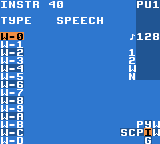
\includegraphics{speech}}
	\end{center}
	\caption{Speech Instrument Screen}
	\label{fig:speech}
\end{figure}
\begin{figure}[htpb]
	\begin{center}
	\fbox{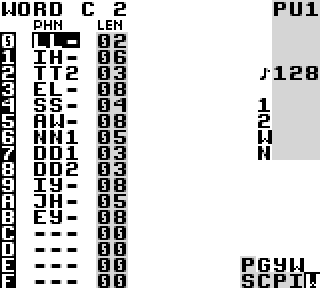
\includegraphics{word}}
	\end{center}
	\caption{Example Word}
	\label{fig:word}
\end{figure}

To edit a word, press \textsc{select+right} to get to the word screen. The left column contains the allophones to be played, the right column sets their duration. The word in figure~\ref{fig:word} is supposed to say ``Little Sound Dj.''

To make the words easy to remember, rename them by tapping A in the speech instrument screen.

\section{Allophones}

\begin{itemize}
\item When selecting allophones, care about how they sound, not how they are spelled.
\item A sound may be different depending on its position within a word. For example, the K in ``coop'' will sound different from the K's in ``keep'' and ``speak''.
\end{itemize}

Allophones marked with * loop indefinitely.

\subsection{Short vowels}

\begin{description}
\item[*IH] sitting, stranded
\item[*EH] extent, gentlemen
\item[*AE] extract, acting
\item[*UH] cookie, full
\item[*AD] talking, song
\item[*AX] lapel, instruct
\end{description}

\subsection{Long vowels}

\begin{description}
\item[IY] treat, people, penny
\item[EY] great, statement, tray
\item[AY] kite, sky, mighty
\item[OI] noise, toy, voice
\item[UW1] after clusters with YY: computer
\item[UW2] in monosyllabic words: two, food
\item[OW] zone, close, snow
\item[AW] sound, mouse, down
\item[EL] little, angle, gentlemen
\end{description}

\subsection{R-colored vowels}

\begin{description}
\item[ER1] letter, furniture, interrupt
\item[ER2] monosyllables: bird, fern, burn
\item[OR] fortune, adorn, store
\item[AR] farm, alarm, garment
\item[YR] hear, earring, irresponsible
\item[XR] hair, declare, stare
\end{description}

\subsection{Resonants}
\begin{description}
\item[WW] we, warrant, linguist
\item[RR1] initial position: read, write, x-ray
\item[RR2] initial clusters: brown, crane, grease
\item[LL] like, hello, steel
\item[YY1] clusters: cute, beauty, computer
\item[YY2] initial position: yes, yarn, yo-yo
\end{description}

\subsection{Voiced fricatives}
\begin{description}
\item[VV] vest, prove, even
\item[DH1] word-initial position: this, then, they
\item[DH2] word-final and between vowels: bathe, bathing
\item[ZZ] zoo, phase
\item[ZH] beige, pleasure
\end{description}

\subsection{Voiceless fricatives}
\begin{description}
\item[*FF] fire, fox
\item[*TH] this, they
\item[*SS] sit, smile
\item[SH] shirt, leash, nation
\item[HH1] before front vowels: YR, IY, IH, EY, EH, XR, AE
\item[HH2] before back vowels: UW, UH, OW, OY, AO, OR, AR
\item[WH] white, whim, twenty
\end{description}

\subsection{Voiced stops}
\begin{description}
\item[BB1] final position: rib; between vowels: fibber, in clusters: bleed, brown
\item[BB2] initial position before a vowel: beast
\item[DD1] final position: played, end
\item[DD2] initial position: down; clusters: drain
\item[GG1] before high front vowels: YR, IY, IH, EY, EH, XR
\item[GG2] before high back vowels: UW, UH, OW, OY, AX; and clusters: green, glue
\item[GG3] before low vowels: AE, AW, AY, AR, AA, AO, OR, ER; and medial clusters: anger; and final position: peg
\end{description}


\subsection{Voiceless stops}
\begin{description}
\item[PP] pleasure, ample, trip
\item[TT1] final clusters before SS: tests, its
\item[TT2] all other positions: test, street
\item[KK1] before front vowels: YR, IY, IH, EY, EH, XR, AY, AE, ER, AX; initial clusters: cute, clown, scream
\item[KK2] final position: speak; final clusters: task
\item[KK3] before back vowels: UW, UH, OW, OY, OR, AR, AO; initial clusters: crane, quick, clown, scream
\end{description}

\subsection{Affricates}
\begin{description}
\item[CH] church, feature
\item[JH] judge, injure
\end{description}

\subsection{Nasal}
\begin{description}
\item[MM] milk, alarm, example
\item[NN1] before front and central vowels: YR, IY, IH, EY, EH, XR, AE, ER, AX, AW, AY, UW; final clusters: earn
\item[NN2] before back vowels: UH, OW, OY, OR, AR, AA
\end{description}



